
%     %%%%%%%%%%%%%%%
%
%     P A C K A G E S
%
%     %%%%%%%%%%%%%%%

\documentclass[11pt, a4paper]{article}
\usepackage{fontspec}
\usepackage{caption}

% DOCUMENT LAYOUT
\usepackage{geometry} 
\geometry{a4paper, textwidth=42em, textheight=70em, marginparsep=0.5em, marginparwidth=3.5em}
\setlength\parindent{0em}
\setlength\parskip{0.75em}
\captionsetup{width=0.8\textwidth}

% FONTS
\usepackage[usenames,dvipsnames]{xcolor}
\usepackage{xunicode}
\usepackage{xltxtra}
\defaultfontfeatures{Mapping=tex-text}
%\setromanfont [Ligatures={Common}, Numbers={OldStyle}, Variant=01]{Linux Libertine O}
%\setmonofont[Scale=0.8]{Monaco}
%%% modified by Karol Kozioł for ShareLaTeX use
\setmainfont[
  Ligatures={Common}, Numbers={OldStyle}, Variant=01,
  BoldFont=LinLibertine_RB.otf,
  ItalicFont=LinLibertine_RI.otf,
  BoldItalicFont=LinLibertine_RBI.otf
]{LinLibertine_R.otf}
\setmonofont[Scale=0.8]{DejaVuSansMono.ttf}

% HEADINGS
\usepackage{sectsty}
\usepackage[normalem]{ulem}
\sectionfont{\mdseries\upshape\Large}
\subsectionfont{\mdseries\scshape\normalsize}
\subsubsectionfont{\mdseries\upshape\large}

\renewenvironment{abstract}{%
{\mdseries\scshape\Large\abstractname}
\vspace{1em}\\
}{\par\noindent}

% LISTINGS
\usepackage{listings}
\usepackage{color}
\usepackage{appendix}


%     %%%%%%%%%%%%%%%
%
%     D O C U M E N T
%
%     %%%%%%%%%%%%%%%


\begin{document}
\title{IAR Task 1 Report}
\author{s1311631, s1346981}
\date{\today}
\maketitle

%       ^v^v^v^v^v^v^v^v^v^v^v^v^v^v^v^v^v^v^v^v^v^v^v^v^v^v^v^v^v^v^v^v^v^v^v^


\begin{abstract}
  Lorem ipsum dolor sit amet, consectetur adipiscing elit. Etiam sodales ullamcorper mi, vitae venenatis ex rhoncus sed. Duis aliquam a felis eget scelerisque. Sed cursus euismod metus eu euismod. Suspendisse feugiat faucibus ex. Donec rutrum ipsum sodales justo posuere, ornare consequat mi varius. Suspendisse convallis ullamcorper lorem, non laoreet orci vestibulum sit amet. Aliquam accumsan odio elit, in pharetra leo semper in. Fusce eget varius felis, at semper est. Aenean molestie at felis et fermentum. Fusce ornare risus magna, ac facilisis odio bibendum nec. Vivamus in eros venenatis, interdum odio ac, mollis risus. Praesent urna eros, egestas in gravida ac.
\end{abstract}

%       ^v^v^v^v^v^v^v^v^v^v^v^v^v^v^v^v^v^v^v^v^v^v^v^v^v^v^v^v^v^v^v^v^v^v^v^


\section{Introduction}

The first assignment entails utilising infra-red distance sensors on the Khepera 
robot to navigate autonomously around an environment, ``without hitting obstacles 
or getting stuck in corners or dead-ends. Second, the Robot should tend to follow long walls, 
keeping a consistent distance away from the wall.'' The Robot is controlled remotely 
controlled by a computer over serial. We have elected to use Python as the 
implementation language for this practical.

As per the Task description, we split the development into two goals, one being obstacle 
avoidance and the other being a wall-following behaviour. Our approach is influenced 
by the demonstrable abilities of reaction-based control in robotics and the BUG 
algorithms \cite{principlesrobot}.

%       ^v^v^v^v^v^v^v^v^v^v^v^v^v^v^v^v^v^v^v^v^v^v^v^v^v^v^v^v^v^v^v^v^v^v^v^


\section{Exploring Methods of Not Hitting Things}

\subsection{Experimenting with PID}

% Commit 5837a4b
% Commit f1258e7
% Commit cc5b195

An 8-dimensional PID controller was implemented over the sensor data, yielding an error 
with respect to the distance from an obstacle per sensor -- Too far, the error motivates 
a movement towards the object; Too close and the error motivates a move away.

We use only the two forward-facing sensors to determine if an obstacle is too close, 
and use the two angled sensors on the front adjacent to them to inform the direction in 
which to turn.

This approach had some promising behaviours: The robot was able to prevent itself 
from hitting an object in its path; Similarly it was able to follow a wall to some degree. 
However, wall following would either oscillate towards the wall, bumping against it or 
depart after following for a short distance. This is due in part to the narrow field 
of view afforded by solely using the forward-facing sensor pair.

In addition, the controller was very sensitive to the tuned gains ${K_p}$, ${K_i}$ \&
${K_d}$ and tended to perform best when ${K_p}$ was much larger than the other gains.
The control is neither continuous nor low-latency, as we used discrete thresholds to 
reactively change behaviour based on the error vector PID produced. This discrete 
behavioural change introduced oscillations and resonances to the system, leading us 
to discard PID in favour of a simpler reactive solution. These issues compound to 
indicate that PID is either ill-suited to the problem or overly complex.



\subsection{Force-Vector Control}

We consider treating each distance sensor reading as a force vector pushing 
the robot along the axis of said sensor. Summing these forces gives us an 
`Intended Direction' resultant vector, which is used to correct the initial 
direction vector away from the obstacle. Distances that are further away than
 a threshold are ignored, to stop the robot from moving erratically in open space.

\begin{figure}[h]
  \begin{center}
    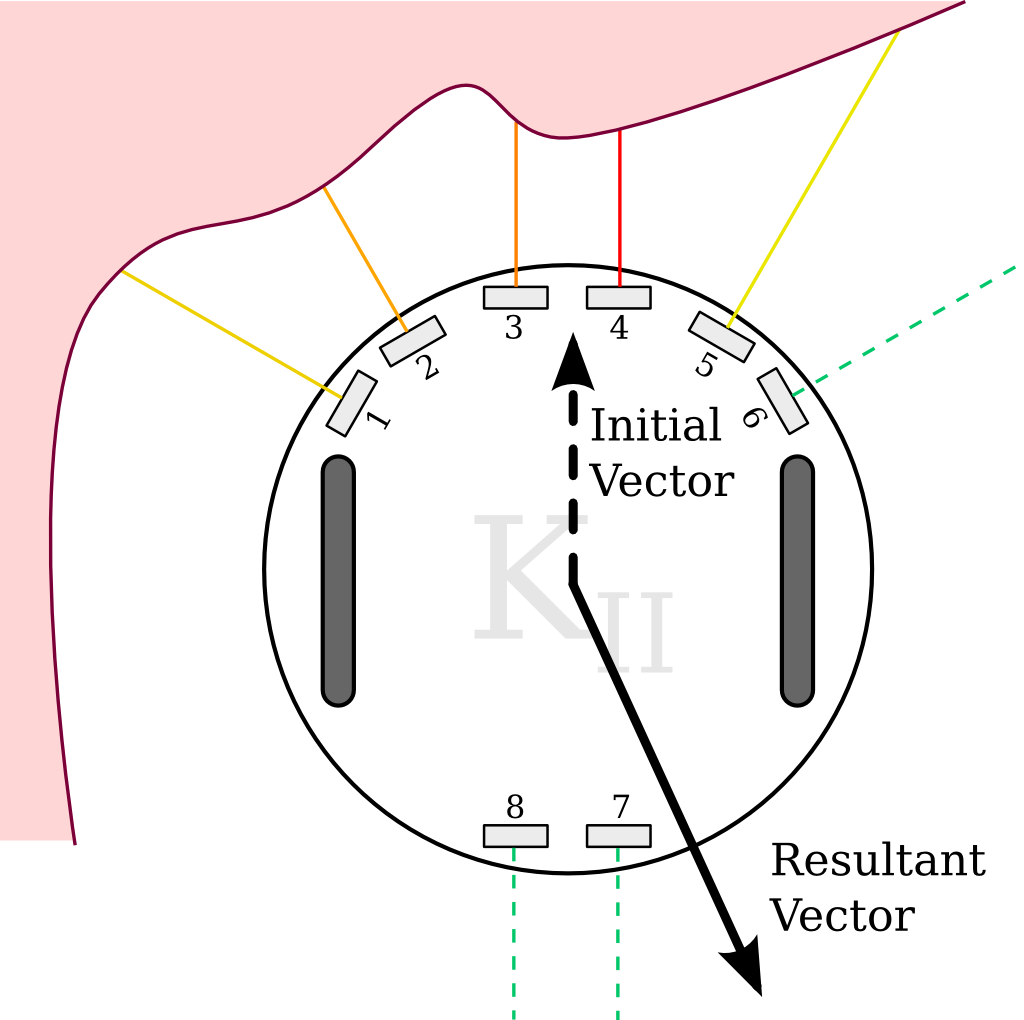
\includegraphics[width=20em]{../assets/force-vector.png}
    \caption{Showing the derivation of Force Vector from distance readings to the
      obstacle; A shorter distance to the obstacle yields a stronger push in the 
      opposite direction. Distances over a threshold (shown dashed) are ignored 
      and have magnitude $0$.}
  \end{center}
\end{figure}

Experimentation that while promising, the lack of calibration between sensors and 
direct mapping to forces introduced a propensity to `wobble', with no exhibition of 
wall-following behaviour as the error vectors push in direct opposition to the wall, 
resulting in an incident-reflection equivalence in the angle the robot takes to the 
wall, basically bouncing off.

Attempts to smooth or condition the sensor signals to prevent wobbling gave the robot 
poor performance in any environment with acute angles and unsmooth edges.

The method is, however, somewhat more elegant than PID \& rule based control insofar 
as the complexity of behaviour that emerges from a simple rule set. Nonetheless, we 
discard Force-Vector control in favour of Reaction-Based control as detailed in the 
following text, using some methods learned from the PID Experiment.

%       ^v^v^v^v^v^v^v^v^v^v^v^v^v^v^v^v^v^v^v^v^v^v^v^v^v^v^v^v^v^v^v^v^v^v^v^


\section{Developing Wall-Following Behaviour}

We observe that distance threshold based obstacle-avoidance does develop some 
wall-following-like behaviour, yet fails to follow \emph{at a constant distance} due 
to the fact it will turn until the wall is no longer in front of it, but has no problem 
with over-correcting by some small angle nor does it's concept of error make it seek 
out a wall to hug.

Our final obstacle-avoidance method reactionally adjusts our trajectory away from a 
collision using a composition of multiple distance sensors, using different groups to 
decide first whether an obstacle is too close, then deciding which way to turn using 
the sensors to choose a direction that presents a larger open-space to move into.
Discrete thresholds are used to make decisions about closeness. When we have made a 
decision to rotate left or right we stick with it until the forward direction is clear; 
this prevents an indecisive oscillation and the robot becoming stuck.

\subsection{Boredom, a useful concept}

The notion that the robot may become `bored' with a wall that it is pursuing gives 
rise to some useful behaviours: If we've failed to identify that we are oscillating 
left and right in a space we may decide to depart, thereby becoming unstuck; Secondly 
an intrinsic property of becoming bored with a wall is that we will not forever circle 
an obstacle thinking it is just a really long wall. This also gives the robot a much 
higher chance of fully exploring it's environment given enough time, as random changes 
in course will continuously occur.

Complete algorithm in pseudo-code/algo style

Source Code is included in the Appendix.

%       ^v^v^v^v^v^v^v^v^v^v^v^v^v^v^v^v^v^v^v^v^v^v^v^v^v^v^v^v^v^v^v^v^v^v^v^


\section{Possible Improvements}

\section{Physical Limitations and Possible Improvements}

The Khepera's distance sensors are spaced to prioritise forward motion, which is handy 
for exploring a space though does make reversing out of a dead-end much harder than 
turning on the spot then driving out forwards.

Evenly spaced sensors

RF Serial on top


%       ^v^v^v^v^v^v^v^v^v^v^v^v^v^v^v^v^v^v^v^v^v^v^v^v^v^v^v^v^v^v^v^v^v^v^v^


\begin{appendices}
\section*{Appendix}
\subsection{Code Listings}
TODO
%\lstinputlisting[language=python]{../../main.py}
\end{appendices}


\begin{thebibliography}{1}

\bibitem{principlesrobot}
Principles of Robot Motion: Theory, Algorithms, and Implementation\\
\textit{Howie Choset}

\end{thebibliography}
\end{document}
